
\section{Preliminaries}
\label{section:Preliminaries}
\subsection{Syntax and Semantics of Boolean Program}
\label{section:SyntaxAndSemanticsOfBooleanProgram}

% 布尔程序是对一般的程序应用谓词抽象之后产生的结果。布尔程序的变量既可以是全局变量,也可以是局部变量。
A boolean program can be considered as a predicate abstraction of its corresponding C program, as all variables in boolean program are of boolean type, representing predicates in the C program. The variables in boolean program can be global or local.
% 在布尔程序中,所有变量均是布尔类型的,因此在声明变量时无需再给出变量的类型。
When declaring a variable in boolean program the type of the variable does not need to be explicitly given, as all of them must be of boolean type.
% 布尔程序中只包含两个常量:0(假)和1(真),同时布尔变量的取值还可以是 不确定。
There are only two literals in boolean program: $0$(\textit{false}) and $1$(\textit{true}), but the value of a variable could also be \textit{uncertain}(represented by $*$).
% 布尔程序中的语句有着与C语言语句类似的结构,允许为某个语句赋予标签。
The statements in boolean program have similar structures with their couterparts in C Labels can also be assigned to arbitary statements.
% 布尔程序还有着与Python类似的并行赋值,允许同时将一组值赋给一组变量
Boolean program also supports parallel assignment like Python, which can be used to assign a tuple of values to another tuple of variables simultaneously.
% 例如,简单的一句 a,b = b,a 即可互换变量a和b的取值
For instance, $a, b = b, a$ can simply swap the values of variable $a$ and $b$.
There are three kinds of statements that can control the execution path of a boolean program: $if$, $while$, $assert$, which have similar functionalities with their counterparts in C.
% 在此,我们给出布尔程序的形式化表示方法。
Next, we shall present the formal definition of a boolean program.

% 首先,我们定义布尔程序的变量的集合为V,其中包括了布尔程序的全局变量及局部变量
First, assume $V$ represents a set of variables in a boolean program, including global variables and local variables.
% 我们将估值\xi\subseteq V定义为程序在某一时刻所能访问到的值为1的变量,并得出\xi的幂集X=2^{V}
Also, we use evaluation $\xi \subseteq V$ to represent the set of accessible $true$ variables in a given moment of the program execution, and we have its power set of $\xi$ being $X = 2^{V}$.
At this point of view, it shall be intuitive to consider the control flow graph of boolean program $B$ as a DFA\footnote{Deterministic Finite Automaton} $A_{B}$, which includes:
\begin{itemize}
\item A finite set of {\it statement}s $S=\{s_{1},s_{2},\dots,s_{n}\}$
\item A finite set of {\it state}s $Q$, where each $q \in Q$ consists of a statement and an evaluation, i.e. $q=(s,\xi)$, meaning the program is going to execute statement $q$, and the values of all variables at this time are described by evaluation $\xi$. A state can be represented as a node in the control flow graph.
\item A transition function $q=next(s,\xi)$, which represent a transition from state $p=(s,\xi)$ to state $q$. If there is a state $p=(s,\xi)$, then $next(p)$ is such a state $q=(s\prime,\xi\prime)$ that if the program execute statement $s$ with evaluation $\xi$, the program will step to statement $s\prime$ with evaluation $\xi\prime$. A transition from state $p$ to state $q$ can be represented as an edge from node $p$ to node $q$ in the control flow graph.
\item An initial state $init \in Q$.
\end{itemize}

Such definition is sufficient for most boolean programs, but it is a little tricky when we try to simulate an invocation of a function.
To address this problem, we use a new automaton to represent the execution of the invoked function, with its initial state determined by the evaluation of its parameters.
The invocation statement and the return of the function trigger transitions from one automaton to another, represented as a dashed edge in the control flow graph.
The inter-automata transitions are transparent to the invoker, as the automaton of invoker function will halt while we are simulating the invoked function, and transfer to its next state according to the result returned by the invoked function.
Formally speaking, assume the automaton of invoker function being $src$ and the automaton of invoked function being $dst$, the edge of invocation would be $\mu:X_{src}\times X_{dst}$. Such mapping assigns the values of arguments to parameters, leaving the values of global variables unchanged, and sets all local variables of the invoked function to {\it uncertain}. Also, we use function $\rho:X_{src}\times X_{dst} \to X_{src}$ to represent the change of evaluation produced by the execution of $dst$. Function $\rho$ copies values of all global variables from the evaluation returned by $dst$, copies values of all local variables from the evaluation that $src$ use to invoke $dst$ and assigns the values returned by $dst$ to the variables designated by the invocation statement.

\begin{figure}
\centering
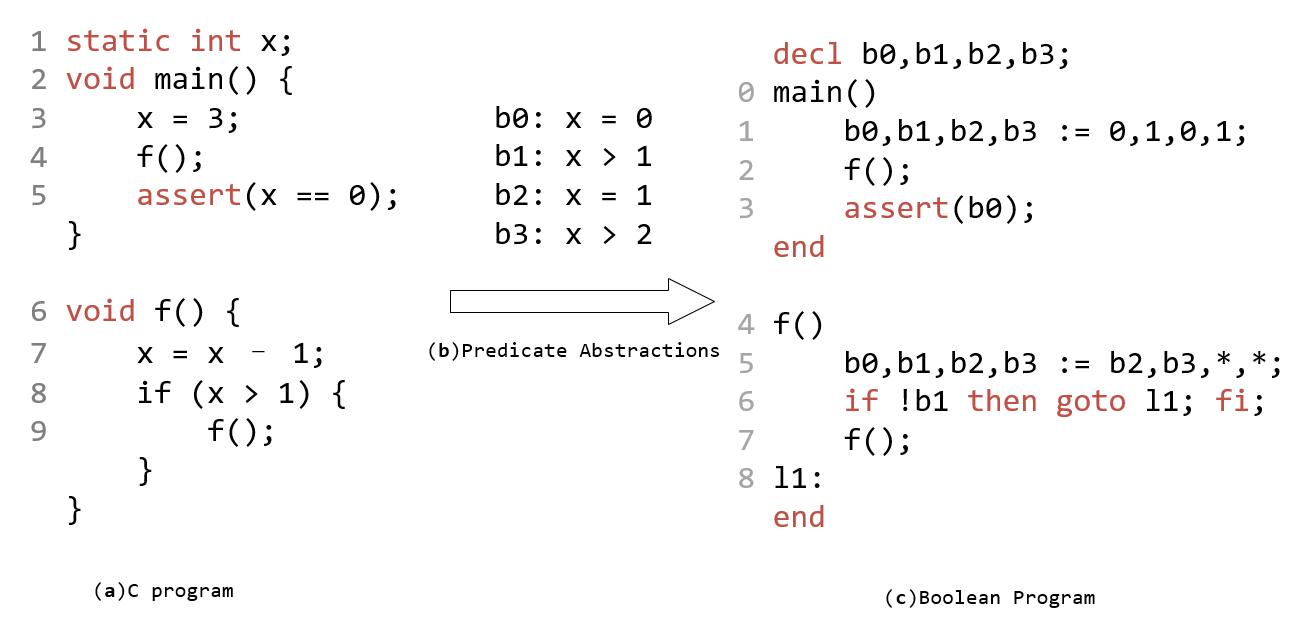
\includegraphics[width=5in,height=2.5in]{Fig2-1.jpg}
\caption{An example of boolean program conversion}
\label{fig:BPC}
\end{figure}

\begin{figure}
\centering
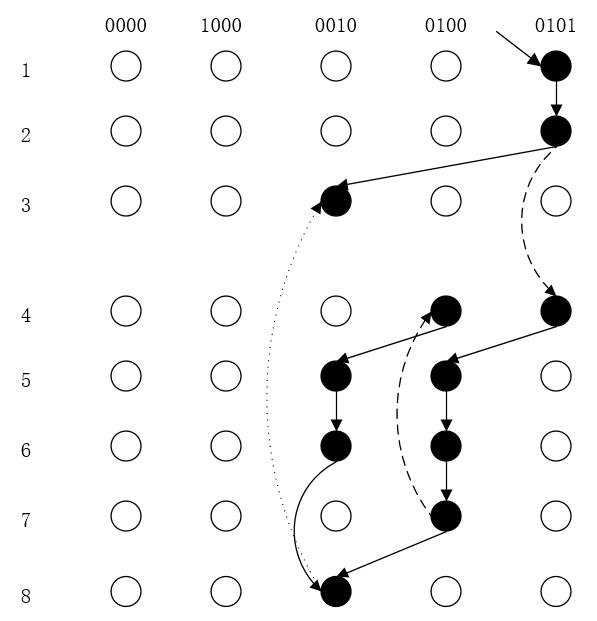
\includegraphics[width=2.5in,height=2.5in]{Fig2-2.jpg}
\caption{The control flow graph}
\label{fig:CFG}
\end{figure}

Takes Figure \ref{fig:BPC} as an example. For the C program in Figure(a), it is obvious that the assertion in line 5 cannot be satisfied. By abstracting the C program using the predicates in Figure(b), the program can be converted to the boolean program in Figure(c). The corresponding control flow graph is shown in Figure \ref{fig:CFG}. Note that the value combinations for $b0$, $b1$, $b2$ and $b3$ can only be $0000$, $1000$, $0010$, $0100$ or $0101$.

\subsection{Constructing Boolean Program}
\label{section:ConstructingBooleanProgram}
% 本文中用于代码修复的布尔程序是通过SATABS对C程序转换得来的。
The boolean program used for program repair in this paper is converted from C program by using SATABS\cite{SATABS}.
% SATBS是一个模型检测的工具,实现了谓词抽象细化循环,它能够将C/C++的程序转换成布尔程序。
SATABS, being a useful tool for model checking, implements iterative predicate abstraction refinement algorithm\cite{CCoCaVUPAaI}, and can be used to convert ANSI-C program to an equivalent boolean program.
% 给定了输入程序之后,SATABS会自动计算出它的抽象表示。为了达到程序的状态空间缩减的目的,抽象是一个很有效的方法。
For a given C program, SATABS will compute for its abstract representation automatically, which is an effective way to reduce the number of states.
% 谓词抽象是其中一种广泛应用的方法,它通过只保持跟踪一定的谓词来抽象数据。在抽象模型中,消去了原程序的变量,以布尔变量来表示根据原程序抽象出来的谓词
Predicate abstraction\cite{CoASGwPVS,GFSAoRSUDP} is one of the most popular abstracting algorithms, which abstracts the program's data by tracking a limited number of predicates.
% 在抽象模型中,消去了原程序的变量,以布尔变量来表示根据原程序抽象出来的谓词。
In the abstract model, variables of the original program will be omitted, and boolean variables will be used to represent the abstracted predicates.
% 抽象程序是通过存在抽象创建的,存在抽象对于可达性属性来说是保守的抽象,也即对于在抽象模型中存在的属性,也一定能在原始程序中找到同样的属性。
% The abstracted program is produced by existential abstraction\cite{MCaA}, which is a pretty conservative abstraction for reachability properties, meaning for every property in the abstracted model, there will always be a corresponding property in the original program.
\subsubsection{Converting an Assignment Statement}
\label{section:ConvertingAnAssignmentStatement}
% SATABS根据具体程序的状态迁移关系计算基本块的抽象迁移关系,得出抽象谓词集合P,每一个布尔变量对应集合P中的一个谓词。
Based on the state transitions of the given program, SATABS can calculate the abstracted state transitions between basic blocks and produce a set of abstracted predicates $P$, with every boolean variable corresponds to one predicate in $P$.
% 在得出谓词集合后进行转换的过程中,若原始程序在位置L处有赋值语句x=e,则布尔程序B在L出将包含对布尔变量的赋值语句[6]。
When the program is being converted, if there used to be an assignment statement, for example $x = e$, at location $L$ in the original program, there will also be an assignment statement for the corresponding boolean variable at location $L$ in the boolean program\cite{MLS:STEPaBP}.
% 布尔变量的真假值根据计算出的抽象状态迁移关系的谓词的真假值进行复制。
Value for the boolean variable is computed based on its corresponding predicate.
% 如果在L处不能确定谓词的真假值,则在B中的布尔变量只表示为:b_i= *。
If the value of the predicate cannot be determined at location $L$, the statement in $B$ will look like $b_{i} = *$, meaning {\it uncertain}.

For example, given the C program in Figure \ref{fig:BPC}(a), the predicate set computed by SATABS is $\{b0 : x = 0, b1 : x > 1, b2 : x = 1, b3 : x > 2\}$. Then it is easy to know the boolean assignment statements for C statements $x = 3$ and $x = x - 1$ will be $b0,b1,b2,b3 := 0,1,0,1$ and $b0,b1,b2,b3 := b2,b3,*,*$.

\subsubsection{Converting a Control Flow Statement}
\label{section:ConvertingAControlFlowStatement}
% 除了由赋值语句组成的初始块,程序中还包括了if、while和for等控制语句。
Except for basic blocks of assignment statements, there are also control flow statements like $if$, $while$ and $for$ in boolean program.
% 这些语句包含作为参数的条件语句,但它们不会改变变量的取值而只会决定控制流的方向 \cite{35}。
Some of them can have conditional expression as their parameter, but they will not change the values of variables: all they do is changing the direction of control flow.
% 表2-1中给出了C语言程序中比较常见的控制语句转换的例子。从表中的3个例子可以总结出C语言程序的控制结构转换为布尔程序的规则。
Table \ref{table:ControlStatementConversions} shows examples of conversions of $C$ control flow statements, one can easily sum up the basic rules behind these conversions by these examples.

\begin{table}
\label{table:ControlStatementConversions}
\center
\begin{tabular}{c|l|c|l}
\hline
Type & C & Predicate & Boolean Program \\
\hline
$if$&
\begin{lstlisting}
if(x>1){
  f();
}
\end{lstlisting}&
\begin{lstlisting}
b1 : x>1
\end{lstlisting}&
\begin{lstlisting}
  if !b1
  then
    goto l1;
  fi;
  f();

l1:
\end{lstlisting} \\
\hline
$while$&
\begin{lstlisting}
while(x>1){
  x=x-1;
}
\end{lstlisting}&
\begin{lstlisting}
b0 : x==0
b1 : x>=1
b2 : x==1
b3 : x>=2
\end{lstlisting} &
\begin{lstlisting}
l1:
  if !b2
  then
    goto l2;
  if;
  b0,b1,b2,b3 :=
      b2,b3,*,*;
  goto l1;
l2:
\end{lstlisting} \\
\hline
$for$&
\begin{lstlisting}
a=2;
for(i=0;i<a;i++){
  x=x-1;
}
\end{lstlisting} &
\begin{lstlisting}
b0 : x==0
b1 : i>=a
b2 : 1+i>=a
b3 : x==1
b4 : a<=0
b5 : a<=1
\end{lstlisting} &
\begin{lstlisting}
  b1,b2,b4,b5 :=
    *,*,0,0;
  b1,b2 := b4,b5
l1:
  if b1
  then
    goto l2;
  if;
  b0,b3 := b3,*;
  b1,b2 := b2,*;
  goto l1;
l2:
\end{lstlisting} \\
\hline
\end{tabular}
\end{table}

% 对于if条件选择,我们假设原始C语言程序在位置L对一个控制条件语句进行判断:如果该控制条件成立,那么程序将会跳转到位置L_T继续执行条件成立时的语句,否则会跳转到位置L_F执行该条件不成立时的语句。
For conditional statement \lstinline|if|, we assume there is such an \lstinline|if| statement at location $L$, evaluating a boolean expression: if the expression is \lstinline|true|, the control flow goes to location $L_{T}$, otherwise it goes to $L_{F}$.
% 转换时,我们需要对控制条件语句进行抽象,首先就需要遍历该语句的语法结构,检查该控制条件语句中的子表达式是否是谓词集合P中的谓词:
During the conversion, we need to abstract the boolean expression. First of all we need to scan the syntactic structure of this expression, examining whether the sub-expressions belong to predicate set $P$:
% 如果是的话,用对应的布尔变量b_i取代控制条件语句中的表达式。
if they are, we replace the sub-expressions with their corresponding boolean variables $b_{i}$.
% SATABS所采用的策略是对转换后的控制条件语句c进行取非,真正在布尔程序中用于判断的条件语句为c:当c成立时,程序将会跳转到位置L_F,即例子(1)中的l1,并结束if表达式;否则,程序将进入位置L_T,即例子中if语句的后续语句,继续执行。
What SATABS does is negating the converted boolean expression $c$: the exact expression that is used in the converted program would be $\overline{c}$. If $\overline{c}$ is \lstinline|true|, the program will go to location $L_{F}$, being the \lstinline|l1| in example (1), and ends the \lstinline|if| statement; otherwise, the program will go to location $L_{T}$, being the statements right after the \lstinline|if| statement in the example.

% while条件循环语句在布尔程序中则被转换成了if条件选择。
As for \lstinline|while| loop, they are converted into \lstinline|if| statements in boolean program.
% 假设原式C语言程序在位置L有一个对条件语句c进行判断的while条件循环语句,转换后的表达式遵循如下规则:若c不成立,程序将跳转到位置L_F;否则,程序跳转至位置L_T,执行完循环体对应的所有语句后重新跳转到位置L。
As usual, we assume there is a \lstinline|while| statement at location $L$ in the original program, evaluating boolean expression $c$. The converted statement follows such rule that: if $c$ is \lstinline|false|, the program will goto location $L_{T}$, exiting the \lstinline|while| loop; otherwise, the program goes to location $L_{T}$, execute the body of the loop, and goes back to location $L$ for the next loop.

% for条件循环语句在布尔程序中同样被转换成了if条件选择。
\lstinline|for| loops are also converted into \lstinline|if| statements in boolean program.
% 本质上,while循环与for循环是相同的,差别仅在于for循环能够同时为循环内部声明局部变量,因此也需要对其所声明的局部变量进行抽象。
Essentially, \lstinline|for| loop and \lstinline|while| loop are similar, the difference is one can declare local variables in the initialization of \lstinline|for| loop, being the variable \lstinline|i| in example (3). Hence, it is necessary for us to abstract these local variables.
% 转换时,for循环的初始化语句被转换为对应的赋值语句后,放在了转换后的if语句的上方。
The initialization of the original \lstinline|for| loop will be placed above the converted \lstinline|if| statement,
% 同时,for循环的增量表达式也被转换为了赋值语句,并被置于标志循环体结束的goto语句上方。
while the afterthought being converted into assignment statement and placed above the \lstinline|goto| statement, which stands for the end of the loop body.

\subsubsection{Converting a Function Invocation}
\label{section:ConvertingAFunctionInvocation}
% 布尔程序对于原始C语言程序中的函数调用将进行保留,因此布尔程序可以很好地展现具体的C语言程序里的函数调用关系。
Converted boolean program will reserve the function invocations from the original $C$ program, by which the boolean program can reflect the correlations of functions in the original $C$ program accurately.
% 函数的调用分为有参数与无参数函数调用,以及有返回值与无返回值函数调用,其中有参数和无参数的函数调用在转换为布尔程序后均被转化为了无参数函数调用。
For $C$ language, there are invocations with and without parameters, and also functions with and without result returned. For parameter, all functions will be converted into its no-parameter equivalence in boolean program.

% 对于无返回值函数的调用,一般情况下被调用函数都是用于对全局变量进行操作,因此函数调用语句本身可以直接转换,即无论函数调用语句是f()还是f(x),转换成布尔程序后均为f()。
For invocation of function with no result returned (\lstinline|void| function), generally such function will only be used to manipulate global variables, hence it would be equivalent to convert them all to invocation of function without parameter, meaning whether they are \lstinline|f()| or \lstinline|f(x)| in the original program, they will all be \lstinline|f()| in the converted boolean program.

% 对于有返回值函数的调用则稍微复杂一些。在转换时,我们需要额外声明一个布尔变量:该布尔变量不表示任何从C语言程序中抽象出来的具体谓词,而是用于表示被调用函数的返回值。
It would be a little tricky when we are dealing with functions with result returned. During the conversion, we need to declare such a boolean variable additionally: it does not stand for any predicates abstracted from the original variables in the $C$ program, but only stands for the returned result of the invoked function.

\begin{figure}
\centering
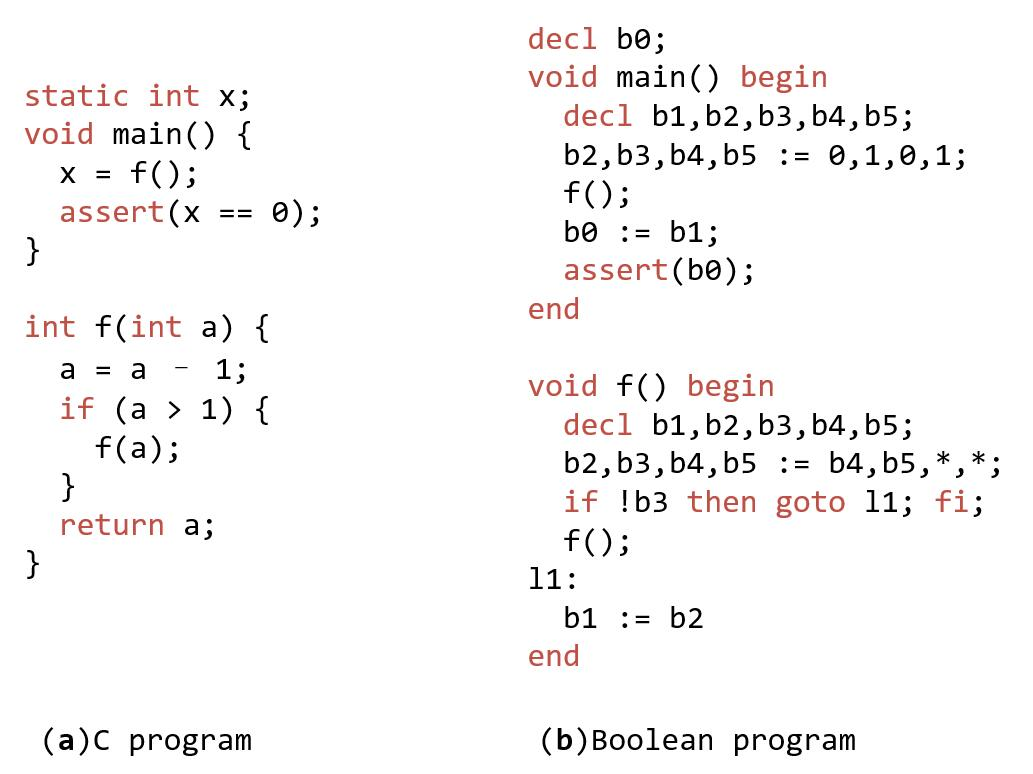
\includegraphics[width=4in,height=3in]{Fig2-3.jpg}
\caption{Another example of boolean program conversion}
\label{fig:BPC_1}
\end{figure}

% 如图2-3中所示的布尔程序,变量b_1代表的便是被调用函数f的返回值。
Figure \ref{fig:BPC_1} shows an example boolean program, in which variable \lstinline|b1| stands for the result returned by function \lstinline|f|.
% 进行函数调用的时候,在调用语句之前,程序会对被调用函数里的局部变量赋初始值,在被调用函数结尾会将返回值赋予该布尔变量,并在调用语句结束后将该布尔变量的值赋予赋值语句所指定的布尔变量。
Before the invocation statement, the converted program will initialize the local variables declared in the invoked function's body, and assign the returning result to the additionally-declared variable at the end of the body.

\subsection{Conjunctive and Disconjunctive Normal Form}
\label{section:CNF_DNF}
In mathematical logic, a \textit{well-formed formula}, often simply \textit{formula}, is a word (i.e. a finite sequence of symbols from a given alphabet) that is part of a formal language.
The formulas of propositional calculus, also called propositional formulas\cite{FOLaATP}, are expressions such as $(A \wedge (B \vee C))$. Their definition begins with the arbitrary choice of a set $V$ of propositional variables. The alphabet consists of the letters in V along with the symbols for the propositional connectives and parentheses "(" and ")", all of which are assumed to not be in V. The formulas will be certain expressions (that is, strings of symbols) over this alphabet.

The formulas are inductively defined as follows:
\begin{itemize}
\item Each propositional variable is, on its own, a formula.
\item If $\varphi$ is a formula, then $\neg \varphi$ is a formula.
\item If $\varphi$ and $\psi$ are formulas, and $\bullet$ is any binary connective, then $\varphi \bullet \psi$ is a formula. Here $\bullet$ could be (but is not limited to) the usual operators $\vee$, $\wedge$, $\to$, or $\leftrightarrow$.
\end{itemize}

In Boolean logic, a formula is in \textit{conjunctive normal form} (CNF) if it is a conjunction of clauses, where a clause is a disjunction of literals; otherwise put, it is an \textit{AND} of \textit{OR}s.
As comparison, a \textit{disjunctive normal form} (DNF) is a standardization (or normalization) of a logical formula which is a disjunction of conjunctive clauses, which can also be described as an \textit{OR} of \textit{AND}s.
For conjunctive and disconjunctive normal form, the only propositional operators are \textit{and}($\wedge$), \textit{or}($\vee$) and \textit{not}($\neg$), where the \textit{not} operator can only be used as part of a literal, meaning it can only precede a propositional variable.

The formal grammar for DNF and CNF can be expressed as follows:

\begin{tabular}{ccc}
$\textit{literal}$ & $\to$ & $\textit{variable}$ \\
$\textit{literal}$ & $\to$ & $\neg \textit{variable}$ \\
$\textit{conjunctive clause}$ & $\to$ & $\textit{literal}$ \\
$\textit{conjunctive clause}$ & $\to$ & $(\textit{literal} \wedge \textit{conjunctive clause})$ \\
$\textit{DNF}$ & $\to$ & $\textit{conjunctive clause}$ \\
$\textit{DNF}$ & $\to$ & $(\textit{conjunctive clause} \vee \textit{DNF})$ \\
$\textit{disjunctive clause}$ & $\to$ & $\textit{literal}$ \\
$\textit{disjunctive clause}$ & $\to$ & $(\textit{literal} \vee \textit{disjunctive clause})$ \\
$\textit{CNF}$ & $\to$ & $\textit{disjunctive clause}$ \\
$\textit{CNF}$ & $\to$ & $(\textit{disjunctive clause} \wedge \textit{CND})$
\end{tabular}

where \textit{variable} can be any variable.

\subsection{Satisfiability Modulo Theories}
\label{section:SatisifiabilityModuloTheories}
Variables in converted boolean program are somehow different from general boolean variables: they all are bound to specific predicates abstracted from the original $C$ program, which provide them {\it meanings}.
With all these meanings behind them, some value combinations would be impossible for them to take, as such combinations result in conflicts on their meanings.
For example, consider a predicate abstraction where $p_{1}$ stands for \lstinline|x == 0| and $p_{2}$ stands for \lstinline|x == 1|.
Combination \lstinline|p1 : true, p2 : true| is impossible as it is impossible for \lstinline|x == 0| and \lstinline|x == 1| both being \lstinline|true| at the same time.
It is important to consider which combinations are possible for a boolean program, as the set of all possible combinations would be generally smaller than $2^{V}$.
Considering other problems in a smaller set can bring great reduction to the search space.
Hence, we introduce satisfiability modulo theories.

In computer science and mathematical logic, the satisfiability modulo theories (SMT) problem\cite{SMT} is a decision problem for logical formulas with respect to combinations of background theories expressed in classical first-order logic with equality.
Formally speaking, an SMT instance is a formula in first-order logic, where some function and predicate symbols have additional interpretations, and SMT is the problem of determining whether such a formula is satisfiable.
In other words, SMT problem can be considered as a SAT\footnote{Boolean satisfiability problem} problem in which some of the binary variables are replaced by predicates over a suitable set of non-binary variables\cite{BSAT:SMT}.

We assume a countable set of variables $X$, function symbols $F$ and predicates $P$.\cite{ToSMT}
A first-order signature $\Sigma$ is a partial map from $F \cup P$ to the natural numbers corresponding to the {\it arity} of the symbol.
A $\Sigma$-{\it term} $\tau$ has the form
\begin{equation}
\label{eq:SigmaTerm}
\tau := x | f(\tau _{1}, \dots, \tau _{n})
\end{equation}
where $f \in F$ and $\Sigma(f) = n$. For example, if $\Sigma(f) = 2$ and $\Sigma(g) = 1$, then $f(x, g(x))$ is a $\Sigma$-term.
A $\Sigma$-{\it formula} has the form
\begin{equation}
\label{eq:SigmaFormula}
\psi := p(\tau _{1}, \dots, \tau _{n}) | \tau _{0} = \tau _{1} | \neg \psi _{0} | \psi _{0} \vee \psi _{1} | \psi _{0} \wedge \psi _{1} | (\exists x : \psi _{0}) | (\forall x : \psi _{0})
\end{equation}
where $p \in P$ and $\Sigma(p) = n$, and each $\tau _{i}$ is a $\Sigma$-term. For example, if $\Sigma(<) = 2$ for a predicate symbol $<$, then $(\forall x : (\exists y : x < y))$ is a $\Sigma$-formula.
A $\Sigma$-{\it structure} $M$ consists of a nonempty domain $|M|$, for each $p \in P$ such that $\Sigma(p) = n$, $M(p)$ is a subset of $|M|^{n}$, and for each $x \in X$, $M(x) \in |M|$.
The interpretation of a term $a$ in $M$ is given by $M\llb x \rrb = M(x)$ and $M\llb f(a_{1},\dots,a_{n})\rrb = M(f)(M\llb a_{1}\rrb\dots M\llb a_{n}\rrb )$.
For a $\Sigma$-formula $\psi$ and a $\Sigma$-structure $M$, satisfaction $M \models \psi$ can be defined as

\emptyline
\begin{center}
\begin{tabular}{rcl}
$M\models a = b$                      & $\Longleftrightarrow$ &   $M\llb a\rrb = M\llb b\rrb$                            \\
$M\models p(a_{1},\dots,a_{n})$       & $\Longleftrightarrow$ &   $(M\llb a_{1}\rrb,\dots,M\llb a_{n}\rrb) \in M(p)$     \\
$M\models\neg\psi$                    & $\Longleftrightarrow$ &   $M\not\models\psi$                                     \\
$M\models \psi _{0}\vee\psi _{1}$     & $\Longleftrightarrow$ &   $M \models\psi _{0}$ or $M\models\psi _{1}$            \\
$M\models \psi _{0}\wedge\psi _{1}$   & $\Longleftrightarrow$ &   $M\models\psi _{0}$ and $M\models\psi _{1}$            \\
$M\models (\forall x : \psi)$         & $\Longleftrightarrow$ &   $M\{x\mapsto a\}\models\psi$, for all $a\in |M|$       \\
$M\models (\exists x : \psi)$         & $\Longleftrightarrow$ &   $M\{x\mapsto a\}\models\psi$, for some $a\in |M|$      \\
\end{tabular}
\end{center}
\emptyline

A first-order $\Sigma$-formula $\psi$ is {\it satisfiable} if there is a $\Sigma$-structure $M$ such that $M \models\psi$, and it is valid if in all $\Sigma$-structures $M$, $M \models\psi$.